\documentclass[11pt,a4paper]{article}

% dyngen

%%%%%%%%%%%%%%%%%%%%%%%
%%% IMPORT PACKAGES %%%
%%%%%%%%%%%%%%%%%%%%%%%

\usepackage[margin=2.5cm,a4paper]{geometry}

% text packages
\usepackage{csquotes}
\usepackage[english]{babel}
\usepackage{setspace}	

% scripting packages
\usepackage{blindtext}

% style packages
\usepackage{lmodern}
\usepackage{fancyhdr}
\usepackage{microtype} % Sublim­i­nal re­fine­ments to­wards ty­po­graph­i­cal per­fec­tion

% figure packages
\usepackage{tikz}
\usetikzlibrary{calc,shapes,arrows,intersections,shadows}
\tikzset{>=latex}
\usepackage{graphicx}
\usepackage[indention=0.5cm,labelsep=colon,font={sf,small},labelfont={bf,sf}]{caption}
\usepackage[indention=0.5cm,font={sf,small},labelfont={bf,sf}]{subcaption}
\usepackage{float}
\usepackage{multirow}
\usepackage{import}
\usepackage{xcolor}
\usepackage{colortbl}

% pseudocode packages
\usepackage{algorithm}
\usepackage{algpseudocode}

% symbols packages
\usepackage{amssymb}
\usepackage{amsmath}

% table packages
\usepackage{tabularx}
\usepackage{tabulary}
\usepackage{booktabs}

% references packages
\usepackage[sorting=none]{biblatex}
\bibliography{library}
\usepackage{bibentry}

% link packages
\usepackage{url}
\usepackage{doi}

% add checkmark commands
\usepackage{pifont}
\newcommand{\cmark}{\ding{51}}
\newcommand{\xmark}{\ding{55}}

% authors and affiliations
\usepackage{authblk}

% command for adding comments
 \newcommand{\mycomment}[1]{\noindent\fbox{\parbox{\textwidth}{\color{red}#1}}}
%\newcommand{\mycomment}[1]{}

%%%%%%%%%%%%%%%%%%%%%%%%%%%%%
%%% DEFINE FIGURE HELPERS %%%
%%%%%%%%%%%%%%%%%%%%%%%%%%%%%

\newcommand{\hugefigure}{\textwidth}
\newcommand{\LARGEfigure}{0.8\textwidth} % 1 per col
\newcommand{\LARgefigure}{0.6\textwidth} % 1 per col
\newcommand{\Largefigure}{0.5\textwidth} % 1 per col
\newcommand{\largefigure}{0.37\textwidth} % 2 per col
\newcommand{\normalfigure}{0.3\textwidth} % 3 per col
\newcommand{\smallfigure}{0.24\textwidth} % 3 per col
\newcommand{\Smallfigure}{0.19\textwidth} % 4 per col
\newcommand{\SMALLfigure}{0.15\textwidth} % 5 per col

%%%%%%%%%%%%%%%%%%%%%
%%% DEFINE STYLES %%%
%%%%%%%%%%%%%%%%%%%%%

\usepackage{fontspec}
\setmainfont [Path = fonts/,
UprightFont = *-300,
ItalicFont = *-300-Italic,
BoldFont = *-700,
BoldItalicFont = *-700-Italic
]{MuseoSans}

%% hyperlinks
\usepackage{hyperref}

\renewcommand{\baselinestretch}{1.25}

\begin{document}

\title{dyngen: benchmarking with \textit{in silico} single cells}

\newcommand{\afdambi}{1}
\newcommand{\afappmat}{2}
\newcommand{\afcmgg}{3}
\newcommand{\afcrig}{4}

\author[\afdambi,\afappmat,\afcmgg,\afcrig,*]{Robrecht~Cannoodt}
\author[\afdambi,\afappmat,*]{Wouter~Saelens}
\author[\afdambi,\afappmat,$\dagger$]{Yvan~Saeys}

\affil[\afdambi]{{\footnotesize Data Mining and Modelling for Biomedicine group, VIB Center for Inflammation Research, Ghent, Belgium}}
\affil[\afappmat]{{\footnotesize Department of Applied Mathematics, Computer Science and Statistics, Ghent University, Ghent, Belgium}}
\affil[\afcmgg]{{\footnotesize Center of Medical Genetics, Ghent University Hospital, Ghent, Belgium}}
\affil[\afcrig]{{\footnotesize Cancer Research Institute Ghent (CRIG), Ghent, Belgium}}
\affil[*]{{\footnotesize Equal contribution}}
\affil[$\dagger$]{{\footnotesize Corresponding author, \href{mailto:yvan.saeys@ugent.be}{yvan.saeys@ugent.be}}}
\date{}

\maketitle


Many articles introducing novel trajectory inference (TI) tools lack quantitative assessment of the accuracy of the method. Instead, they rely on anecdotal evidence to demonstrate their added value. A brief review of 75 articles reveals that only about 37\% contain a self-assessment (Figure \ref{fig:benchmarks_over_time}A,B). Peer-reviewed articles fared even worse, self-assessing in only 34\% of cases (n=55), whereas articles first published as a pre-print self-assess in 43\% of cases (n=39).

The number of datasets used and methods compared against is also below expectations (Figure \ref{fig:benchmarks_over_time}C,D). Only three TI articles feature a comparison of at least 5 methods using 5 datasets or more \cite{sharma_forksfindingorderings_2017,guo_hoplandsinglecellpseudotime_2017,parra_reconstructingcomplexlineage_2018}.

While self-assessments are universally biased in favour of the authors\cite{norel_selfassessmenttrapcan_2011} (intentially or not), it is dangerous and unusual to publish a computational tool without quantitatively demonstrating its performance compared to state-of-the-art methods. Indeed, a recent comparison of 45 TI methods demonstrated that most methods perform worse than a few baseline methods constructed by combining simple off-the-shelf algorithms such as PCA, $k$-means and MST\cite{saelens_comparisonsinglecelltrajectory_2019}.

In this perspective, we hypothesise that low self-assessment rates are primarily caused by a lack of a standardised problem definition, readily available benchmarking datasets, and suitable metrics. 
We elaborate on these causal reasons, and provide viable solutions for performing TI benchmarks more easily.

\begin{figure}[htb!]
	\centering
	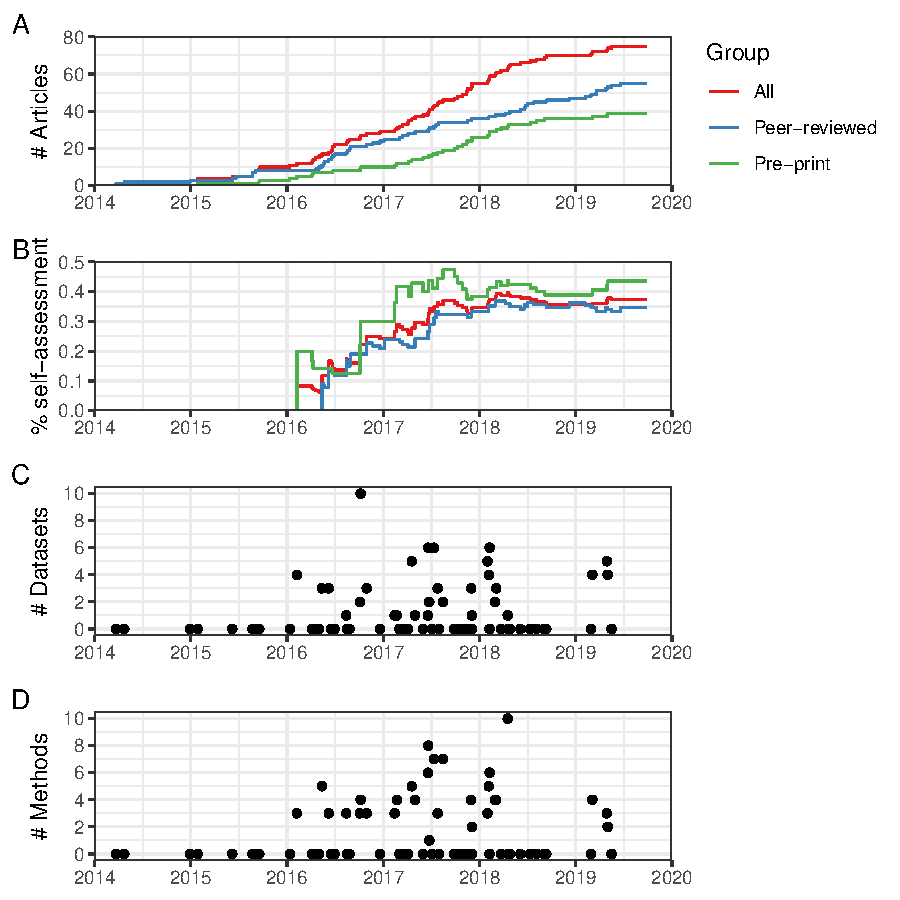
\includegraphics[width=.75\linewidth]{fig/self_assessment.pdf} 
	\caption{
		\textbf{Less than half of all TI articles perform quantitative self-assessment.} 
		\textbf{A:} Since 2016, the number of TI articles has been increasing rapidly. Note that TI methods with both a pre-print and a peer-reviewed article only count once in the overall tally.
		\textbf{B:} Less than 50\% of articles feature a self-assessment. Peer-reviewed articles self-assess only in 34\% of cases.
		\textbf{C:} The number of datasets used in each benchmark is low.
		\textbf{D:} The number of methods (inclusing itself) evaluated is low.
	}
	\label{fig:benchmarks_over_time}
\end{figure}

\section{Problem definition}
One main reason why benchmarking TI methods is difficult is due to there being slight variations 
of the problem a method is attempting to solve (Figure \ref{fig:method_types}A). For example, a method might infer linear or cyclic trajectories, or predict the probability of a cell ending up in one of several end states.

As a result, it becomes harder to discover similar methods to compare against, as certain articles might only show up with search terms such as "pseudotemporal ordering", "lineage trees" or "fate bias". For the discoverability of a new TI method, it is therefore essential to use the term "trajectory inference", or at least list it as one of the keywords. 

\begin{figure}[htb!]
	\centering
	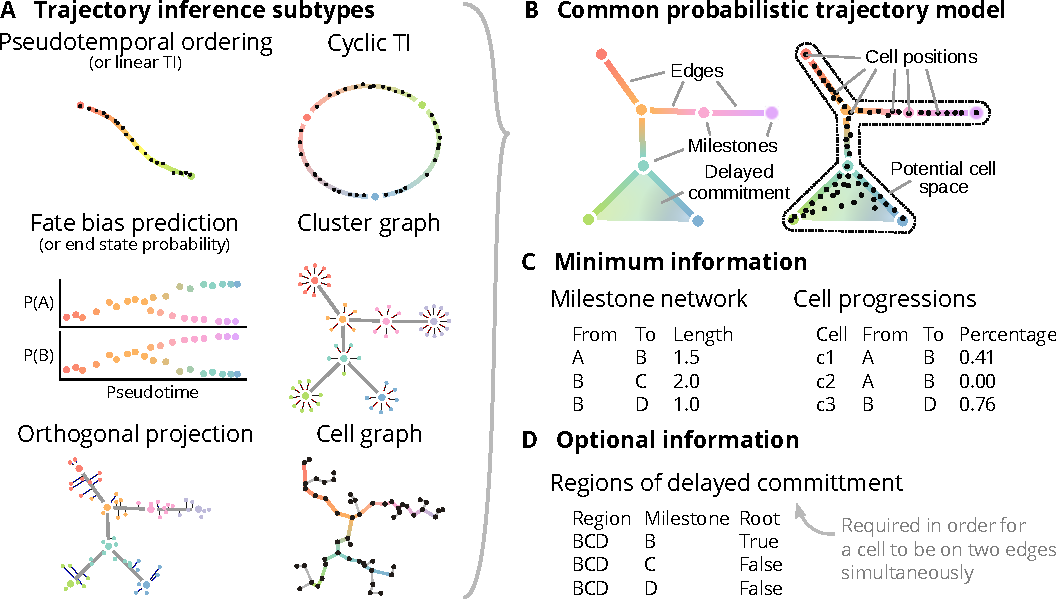
\includegraphics[width=\linewidth]{fig/method_types.pdf} 
	\caption{
		\textbf{Different forms of trajectory inference.}
		\textbf{A:} All TI methods can be categorised in one of seven subtypes in terms of its produced output \cite{saelens_comparisonsinglecelltrajectory_2019}.
		\textbf{B:} Each of these can be translated into a common format, allowing easier comparison of multiple trajectories.
		\textbf{C:} The minimum information required to describe a trajectory in this way is the milestone network -- representing transitions between cellular states -- and the cell progressions -- representing the positions of cells along the transitions.
		\textbf{D:} Optionally, regions of delayed commitment can be defined. A region of delayed commitment contain multiple transitions starting from the same milestone. This allows a TI method to assign probabilities on how likely a cell is part of one of these transitions.
	}
	\label{fig:method_types}
\end{figure}

A more significant and harder to solve problem is that the data formats produced by different methods varies greatly. This makes visualising and comparing multiple trajectories difficult, as different output types cannot be compared directly. The most commonly used and general is one where cells are positioned along a set of edges connecting milestones ("Regular TI", Figure~\ref{fig:method_types}A). 
By adding an extension to regular TI to allow for cells to be part of three or more cellular states, thereby a cell to delay its commitment toward a particular end state (Figure~\ref{fig:method_types}B). 

By adding this extension, all TI subtypes can easily be converted into the common format. Implementations of these conversions can be found in \texttt{dynwrap}\cite{dyno}. Using this standardised format allows developing reusable software for visualising and comparing trajectories from different TI methods.

In practice, this format consists of two data structures: the milestone network specify transition between cell states, and the cell progressions specify how far along each cell has progressed along a transition (Figure~\ref{fig:method_types}C). In addition, regions of delayed commitment need to be specified, if any (Figure~\ref{fig:method_types}D). 

\mycomment{examples? elaborate? citation?}

\section{Benchmarking datasets}
Another hurdle in benchmarking trajectory inference methods is collecting datasets to benchmark against. Before 2018, there were only a handful of datasets containing complex trajectories (Figure~\ref{fig:datasets}). 

When real data is scarce, synthetic data is often used to evaluate computational methods, either standalone (n=5) or to complement real data (n=7). Most synthetic data is generated by the authors themselves (n=8), whereas some reuse datasets generated by others (n=3) or use one of the readily available simulators (n=2). To avoid introducing self-assessment bias in a benchmark, it is recommended to use readily available simulators if they fit the requirements. Examples are dyntoy \cite{saelens_comparisonsinglecelltrajectory_2019}, dyngen \cite{dyngen}, splatter \cite{zappia_splattersimulationsinglecell_2017}, and PROSSTT \cite{papadopoulos_prossttprobabilisticsimulation_2018}.

\begin{figure}[htb!]
	\centering
	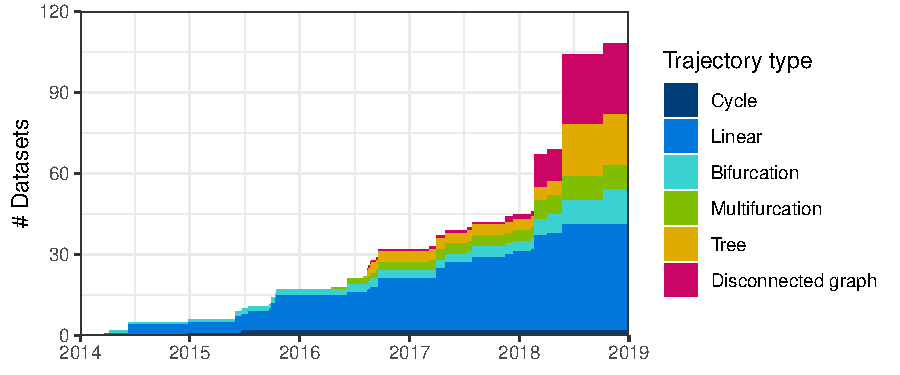
\includegraphics[width=.75\linewidth]{fig/datasets.pdf} 
	\caption{\textbf{An overview collection of real TI benchmarking datasets in function of their publication date and the topology of the trajectory.} These datasets are readily available on Zenodo\cite{cannoodt_singlecellomicsdatasets_2018}.}
	\label{fig:datasets}
\end{figure}

Benefits of synthetic data are that they offer more control over the data characteristics, and that they can be generated in large quantities. This allows to evaluate performance of a method in function of a changing parameter (e.g. dataset size or noise levels), which provides information on how well the method will work on real datasets.

A common counterargument of synthetic data is that they generate unrealistic datasets and thus provide no additional value in evaluation a method. In contrast, we argue that a good set of synthetic datasets should allow benchmarkers to verify that a method should \textit{at least} work well on the synthetic datasets, but good performance on synthetic datasets does not guarantee good performance on real datasets.

Several authors use mainly real datasets to evaluate their method, though only few use more than four datasets (n=7). 
By now, already hundreds of suitable real datasets are available from GEO and ArrayExpress (Figure~\ref{fig:datasets}). Downloading and pre-processing them requires a significant time investment, but by processing the datasets once and storing them in a single repository they can be reused for multiple purposes.

Readers are welcome to reuse (and extend) the 110 real and 229 synthetic datasets used in our comparison of TI methods. The datasets are hosted on Zenodo\cite{cannoodt_singlecellomicsdatasets_2018} and the scripts to process them on GitHub\footnote{\href{https://github.com/dynverse/dynbenchmark/tree/master/scripts/01-datasets}{github.com/dynverse/dynbenchmark/tree/master/scripts/01-datasets}}. Note that the ground truths of the datasets are represented using the common data structures format in the previous section.



\section{Multiple metrics}
The largest problem, by far, seems to be a lack of standardised metrics to evaluate TI methods. None of the benchmarks use a metric directly aimed at comparing the topology or pairwise orderings of two trajectories. 

Instead, most benchmarks (n=26) employ an ordering metric (e.g. pearson correlation) the pseudotime\footnote{The pseudotime value of is calculated by computing its distance from a pre-defined or inferred start cell.} of the predicted trajectory to ground truth information such as the cell type or time of sampling. Several benchmarks (n=5) use a clustering metric (e.g. ARI) to compare a cell's transition assignment or milestone assignment to the ground truth cell type. In four cases, multiple executions were compared to evaluate the robustness of the predictions.
In one particular instance, the pseudotime correlation metric was adapted to be suitable for comparing rooted trees\cite{street_slingshotcelllineage_2018}. In another, an internal measure is used to quantify the smoothness of gene expression along the pseudotime \cite{darocha_reconstructioncomplexsinglecell_2018}.

While each of these metrics provide some insight the correctness of cell orderings or cell clusterings, they do not evaluate the correctness of the prediction's topology. Using only a pseudotime-based metric to evaluate non-linear trajectories is particularly risky, as it 

\begin{figure}[htb!]
	\centering
	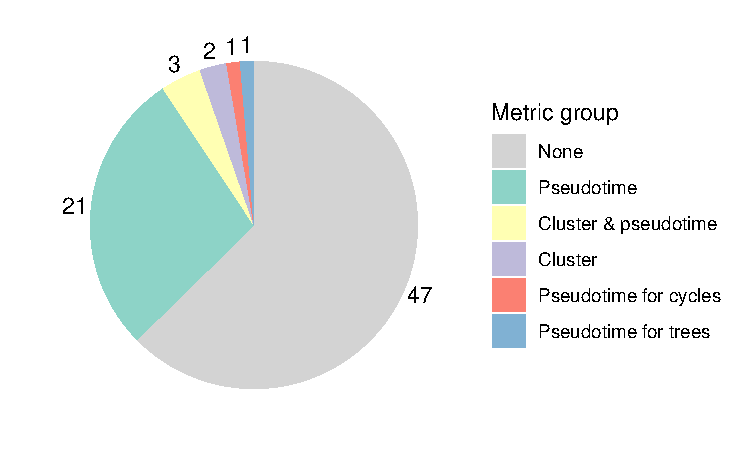
\includegraphics[width=.5\linewidth]{fig/metrics.pdf} 
	\caption{}
	\label{fig:metrics}
\end{figure}

\section{Further guidelines}



\end{document}
